\documentclass[a4paper]{article}
% \usepackage[colorlinks,linkcolor=black,urlcolor=black]{hyperref}
\usepackage{float}
\usepackage{mhchem}
\usepackage{pdfpages}
\usepackage{enumerate}
\usepackage{amsmath}
\usepackage{amssymb}
\usepackage{graphicx}
\usepackage{subfigure}
\usepackage{wrapfig}
\usepackage{geometry}
\usepackage{makecell}
\usepackage{indentfirst}
\usepackage{pdfpages}
\usepackage{multirow} 
\geometry{left=2cm,right=2cm,top=2.5cm,bottom=2.8cm}
\setlength{\parindent}{2em}
\usepackage[greek,english]{babel} 
\makeatletter
\def\@Exercisenum{0}
\newcommand\Exercisenum[1]{
	\def\@Exercisenum{#1}
}
\def\@group{1}
\newcommand\group[1]{
	\def\@group{#1}
}
\newif\iffellowornot\fellowornotfalse
\newcommand\fellow[2]{
	\def\@fellowname{#1}
	\def\@fellowID{#2}
	\fellowornottrue
}
\RequirePackage{titlesec}
\newcommand{\HRule}{\rule{\linewidth}{0.5mm}}
\renewcommand{\maketitle}{
	\begin{titlepage}
	\begin{center}
	\HRule \\[0.8cm]
	\textsc {UM-SJTU Joint Institute \\ Physicis Laboratory II\\(VP241)}\\[0.5cm]
	\HRule \\
	\vfill
	\textsc {Laboratory Report} \\[1.5cm]
	\textsc {Exercise \@Exercisenum} \\[0.8cm]
	\textsc \@title \\ 
	\vfill
	Name: \textbf {Wang Dawei} \ \ \ \ \ ID: 518370910063\ \ \ \ \ \ Group: \@group   
	\iffellowornot
	\\ Name: \@fellowname\ \ \ \ ID: \@fellowID\ \ \ \ \ \ Group: \@group
	\fi
	
	Date: \today 
	\newpage
	\end{center}
	\end{titlepage}
}
\makeatother
\title{The Hall Probe: Characteristics and Applications}
\group{19}
\Exercisenum{2}
\begin{document}
    \maketitle
    \section{Introduction}
    \subsection{Hall Effect}
    \paragraph{} Consider a conducting sheet (made of a metal or a semiconductor) placed in a magnetic field so that the plane of the sheet is perpendicular to the direction of the magnetic field B (Figure \ref{fig:halleffect}). When the electric current $I$ passes through the sheet in the direction shown in Figure \ref{fig:halleffect}, an electric potential difference between the sides $a$ and $b$ of the sheet is generated. The corresponding electric field is perpendicular to both the direction of the current and the direction of the magnetic field. This effect is known as the Hall effect, and the electric potential difference is called the Hall voltage $U_H$.
    \begin{figure}[H]
        \centering
        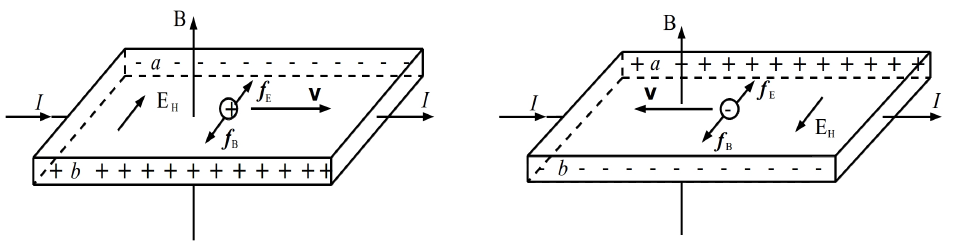
\includegraphics[width=0.8\textwidth]{fig/halleffect.png}
        \caption{The Principle of Hall Effect}
        \label{fig:halleffect}
    \end{figure}
    \paragraph{} The origin of the Hall Voltage comes from the Lorentz force $\textbf{F}_B$. It is perpendicular to the magnetic field and the moving direction of the charge carring particle. So the particles' moving direction is deviated, and consequently an electric field is generated. The electric field also imposes a force upon the particles. In the end, the electric force balances the Lorentz force and a stablized Hall voltage is generated.
    \vspace{-5mm}
    \paragraph{} When the external magnetic field is not very large, the Hall Voltage is proportional to both the current and the magnitude of the magnetic field, and inversely proportional to the thickness of the sheet $d$: 
    \begin{equation}
        U_H=R_H\frac{IB}{d}=KIB,
        \label{eqn:Halleffect}
    \end{equation}
    where $R_H$ is the so-called Hall coefficient and $K=R_H/d=K_H/I$, where $K_H$ is the so-called sensitivity of the Hall element. 
    \subsection{Integrated Hall Probe}
    \paragraph{} The magnitude of the magnetic field can be found by measuring the Hall voltage with a Hall probe when the sensitivity $K_H$ and the current $I$ are fixed. Since the Hall Voltage  is usually very small, it should be amplified after it is measured. Silicon can be used to design both the Hall probe and the integrated circuits, so it is convenient to arrange the Hall probe and the electric circuits into a single device. Such a device is called an integrated Hall probe.
    \vspace{-5mm}
    \paragraph{} The integrated Hall probe SS495A is made up of a Hall sensor, an amplifier and a voltage compensator (Figure \ref{fig:hallprobe}). The relation between the output voltage $U$ and the magnitude of the magnetic field is 
    \begin{equation}
        B=\frac{U-U_0}{K_H}\label{eqn:hallprobe}
    \end{equation}
    \begin{figure}[!ht]
        \centering
        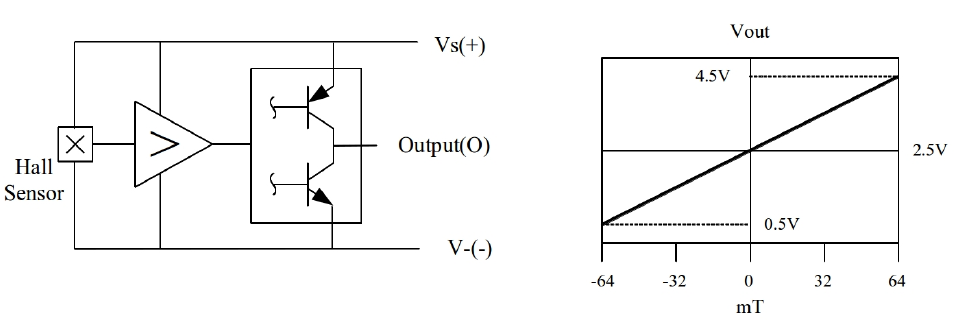
\includegraphics[width=0.8\textwidth]{fig/hallprobe.png}
        \caption{The Circuit Inside the Integrated Hall Probe SS495A(Left). The Relation between the Output Voltage $U$ and the Magnitude of the Magnetic Field $B$(Right).}
        \label{fig:hallprobe}
    \end{figure}
    \subsection{Magnetic Field Distribution Inside a Solenoid}\label{sec:inside}
    \paragraph{} The magnetic field distribution on the axis of a single layer solenoid can be calculated from the following formula \begin{equation}
        B(x)=\mu_0\frac{N}{L}I_M\left\{\frac{L+2x}{2\sqrt{D^2+(L+2x)^2}}+\frac{L-2x}{2\sqrt{D^2+(L-2x)^2}}\right\}=C(x)I_M,\label{eqn:BandI}
    \end{equation}
    where $N$ is the number of turns of the solenoid, $L$ is its length, $I_M$ is the current through the solenoid wire, and $D$ is the solenoid's diameter. The magnetic permeability of vacuum is $\mu_0=4\pi\times 10^{-7}\ \rm H/m$.
    \vspace{-5mm}
    \paragraph{} Based on the information given in the manual, the theoretical magnitude of the magnetic field at the center of the solenoid when $I_M=0.1$A is $B=1.4366$[mT](The uncertainty of this data is zero). Table \ref{tab:theoretical} lists the theoretical value of the magnitude of the magnetic field when $I=0.1$A. 
    \begin{table}[H]
        \centering
        \begin{tabular}{|c|c||c|c|}
            \hline
            $x$[cm]&$B$[mT]&$x$[cm]&$B$[mT]\\\hline
            $\pm 0.0$&1.4366&$\pm 8.0$&1.4057\\\hline
            $\pm 1.0$&1.4363&$\pm 9.0$&1.3856\\\hline
            $\pm 2.0$&1.4356&$\pm 10.0$&1.3478\\\hline
            $\pm 3.0$&1.4343&$\pm 11.0$&1.2685\\\hline
            $\pm 4.0$&1.4323&$\pm 11.5$&1.1963\\\hline
            $\pm 5.0$&1.4292&$\pm 12.0$&1.0863\\\hline
            $\pm 6.0$&1.4245&$\pm 12.5$&0.9261\\\hline
            $\pm 7.0$&1.4173&$\pm 13.0$&0.7233\\\hline
        \end{tabular}
        \caption{Theoretical Value of the Magnetic Field inside the Solenoid}
        \label{tab:theoretical}
    \end{table}
    \section{Apparatus \& Measurement Procedure}
    \subsection{Apparatus}
    \paragraph{}The experimental setup shown in Figure \ref{fig:measure} consists of an integrated Hall probe SS495A (see Figure \ref{fig:Shall}) with $K_H = 31.25 \pm 1.25$ [V/T] (at the working voltage 5 V), a solenoid, a power supply, a voltmeter, a DC voltage divider, and a set of connecting wires.
    \begin{figure}[H]
        \centering
        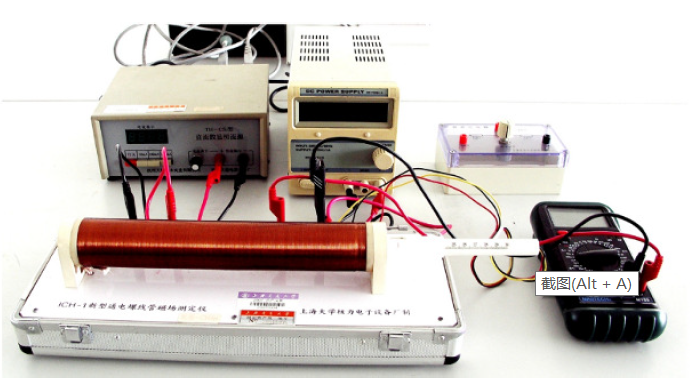
\includegraphics[width=0.5\textwidth]{fig/measurement.png}
        \caption{Measurement Setup}
        \label{fig:measure}
    \end{figure}
    \begin{figure}[H]
        \centering
        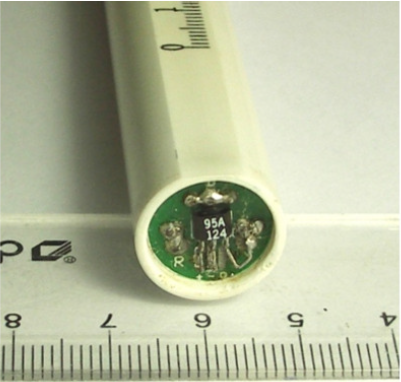
\includegraphics[width=0.3\textwidth]{fig/Shall.jpg}
        \caption{Integrated Hall probe SS495A.}
        \label{fig:Shall}
    \end{figure}
    \begin{table}[H]
        \begin{center}
            \begin{tabular}{|c|c|}
                \hline
                Physical Quantity&Uncertainty\\\hline
                Voltage source&0.5\%[V]\\\hline
                Distance&0.05[cm]\\\hline
                Current source&2\%[mA]\\\hline
                Voltmeter&$0.05\%+6\times 10^{-3}\text{ or }6\times10^{-4}$[V]\\\hline
            \end{tabular}
            \caption{The Uncertainty of the Equipment Used in the Lab}
            \label{tab:uncertainty}
        \end{center}
    \end{table}
    \subsection{Measurement Procedure}
    \subsubsection{Relation Between Sensitivity \(K_H\) and Working Voltage \(U_S\)}
    \begin{enumerate}
        \item I first placed the integrated hall probe at the center of the solenoid(let the reading on the solenoid be 13[cm]). Then I set the working voltage to be $U_S=5$[V] and measured the output voltage $U_0(I_M=0)$ and $U(I_M=250\rm [mA])$. Then I took the theoretical value of $B(x = 0)$ from Section \ref{sec:inside} and calculated the sensitivity of the probe $K_H^*$ using Equation \ref{eqn:hallprobe}.
        \item Then I measured $K_H$ for different values of $U_S$ (from 2.8 V to 10 V) and calculated $K_H/U_S$ and plotted the curve $K_H/U_S$ vs. $U_S$.
    \end{enumerate}
    \subsubsection{Relation Between Output Voltage $U$ and Magnetic Field $B$}
    \begin{enumerate}
        \item I first let the input current to be zero so that $B=0$ and the working voltage $U_S=5$[V], while the probe remains to be at the center of the solenoid. Then I connected the 2.4-2.6V output terminal of the DC voltage divider and the negative port of the voltmeter. Then I adjust the resistance of the divider until the output voltage is 0.
        \item Then I measured the output voltage $U$ for different values of $I_M$ ranging from 0 to 500mA, with intervals of 50mA.
    \end{enumerate}
    \subsubsection{Magnetic Field Distribution Inside the Solenoid}
    \begin{enumerate}
        \item I set the input current $I_M=250$[mA], and then I recorded the output voltage $U$ and the corresponding position $x$.
    \end{enumerate}
    \section{Result}
    \subsection{Relation Between Sensitivity \(K_H\) and Working Voltage \(U_S\)}\label{sec:1}
    \paragraph{} Table \ref{tab:KH*} and \ref{tab:origin1} are two original data tables for this section. We first need to calculate the magnetic field in the center of the solenoid when $I_M=250[\rm mA]$: $$B=B'\frac{I_M}{I_0}=1.4366\times 10^{-3}\times \frac{250}{100}=0.00359[\rm T]\pm 0.00007[T].$$ 
    \begin{table}[H]
        \centering
        \begin{tabular}{|c|c|c|c|c|c|}
            \hline
            $U_S$[V]&Uncertainty[V]&$U_0(I_M=0)$[V]&Uncertainty[V]&$U(I_M=250\rm mA)$[V]&Uncertainty[V]\\\hline
            5.00&0.003&2.472&0.007&2.599&0.007\\\hline
        \end{tabular}
        \caption{The Original Data for $K_H^*$}
        \label{tab:KH*}
    \end{table}
    \begin{table}[H]
        \centering
        \begin{tabular}{|c|c|c|c|c|c|}
            \hline
            $U_S$[V]&Uncertainty[V]&$U_0$[V]&Uncertainty[V]&$U$[V]&Uncertainty[V]\\\hline
            2.840&0.014&1.4004&0.0013&1.4689&0.0013\\\hline
            3.200&0.016&1.5777&0.0014&1.6552&0.0014\\\hline
            3.660&0.018&1.8076&0.0015&1.8963&0.0015\\\hline
            4.04&0.02&1.9969&0.0016&2.0946&0.0016\\\hline
            4.38&0.02&2.161&0.007&2.266&0.007\\\hline
            4.80&0.02&2.373&0.007&2.489&0.007\\\hline
            5.23&0.03&2.584&0.007&2.711&0.007\\\hline
            5.63&0.03&2.785&0.007&2.919&0.007\\\hline
            6.01&0.03&2.971&0.007&3.107&0.008\\\hline
            6.43&0.03&3.175&0.008&3.321&0.008\\\hline
            6.80&0.03&3.362&0.008&3.515&0.008\\\hline
            7.26&0.04&3.583&0.008&3.736&0.008\\\hline
            7.65&0.04&3.778&0.008&3.940&0.008\\\hline
            8.07&0.04&3.984&0.008&4.152&0.008\\\hline
            8.39&0.04&4.140&0.008&4.310&0.008\\\hline
            8.95&0.04&4.418&0.008&4.592&0.008\\\hline
            9.42&0.05&4.647&0.008&4.826&0.008\\\hline
            9.92&0.05&4.889&0.008&5.075&0.009\\\hline
        \end{tabular}
        \caption{The Original Data}
        \label{tab:origin1}
    \end{table}
    Then we calculate the value of $K_H^*$ using data in Table \ref{tab:KH*}. $$K_H^*=\frac{U-U_0}{B}=\frac{2.599-2.472}{0.00359}=35[\rm V/T]\pm 3[V/T].$$
    Then we calculate the value of $K_H$ using data in Table \ref{tab:origin1} and get the data in Table \ref{tab:KHvsUS}. For example, when $U_0=1.4004$[V], $U=1.4689$[V], $U_S=2.840$[V], 
    \begin{eqnarray*}
        K_H=\frac{U-U_0}{B}=\frac{1.4689-1.4004}{0.00359}=19.1[{\rm V/T}]\pm 0.6[{\rm V/T}]\\
        \frac{K_H}{U_S}=\frac{19.1}{2.84}=6.7[{\rm T}^{-1}]\pm 0.2[{\rm T}^{-1}]
    \end{eqnarray*}
    \begin{table}[H]
        \centering
        \begin{tabular}{|c|c|c|c|c|c|}
            \hline
            $K_H$[V/T]&Uncertainty[V/T]&$K_H/U_S$[T$^{-1}$]&Uncertainty[T$^{-1}$]&$U_S$[V]&Uncertainty[V]\\\hline
            19.1&0.6&6.7&0.2&2.840&0.014\\\hline
            21.6&0.7&6.8&0.2&3.200&0.016\\\hline
            24.7&0.8&6.7&0.2&3.660&0.018\\\hline
            27.2&0.8&6.7&0.2&4.04&0.02\\\hline
            29&3&6.6&0.7&4.38&0.02\\\hline
            32&3&6.7&0.6&4.80&0.02\\\hline
            35&3&6.7&0.6&5.23&0.03\\\hline
            37&3&6.6&0.5&5.63&0.03\\\hline
            38&3&6.3&0.5&6.01&0.03\\\hline
            41&3&6.4&0.5&6.43&0.03\\\hline
            43&3&6.3&0.4&6.80&0.03\\\hline
            43&3&5.9&0.4&7.26&0.04\\\hline
            45&3&5.9&0.4&7.65&0.04\\\hline
            47&3&5.8&0.4&8.07&0.04\\\hline
            47&3&5.6&0.4&8.39&0.04\\\hline
            48&3&5.4&0.3&8.95&0.04\\\hline
            50&3&5.3&0.3&9.42&0.05\\\hline
            52&4&5.2&0.4&9.92&0.05\\\hline
        \end{tabular}
        \caption{The Data for $K_H$ vs. $U_S$.}
        \label{tab:KHvsUS}
    \end{table}
    Using the last four columns of Table \ref{tab:KHvsUS}, I obtained Figure \ref{fig:KHvsUS}.
    \begin{figure}[H]
        \centering
        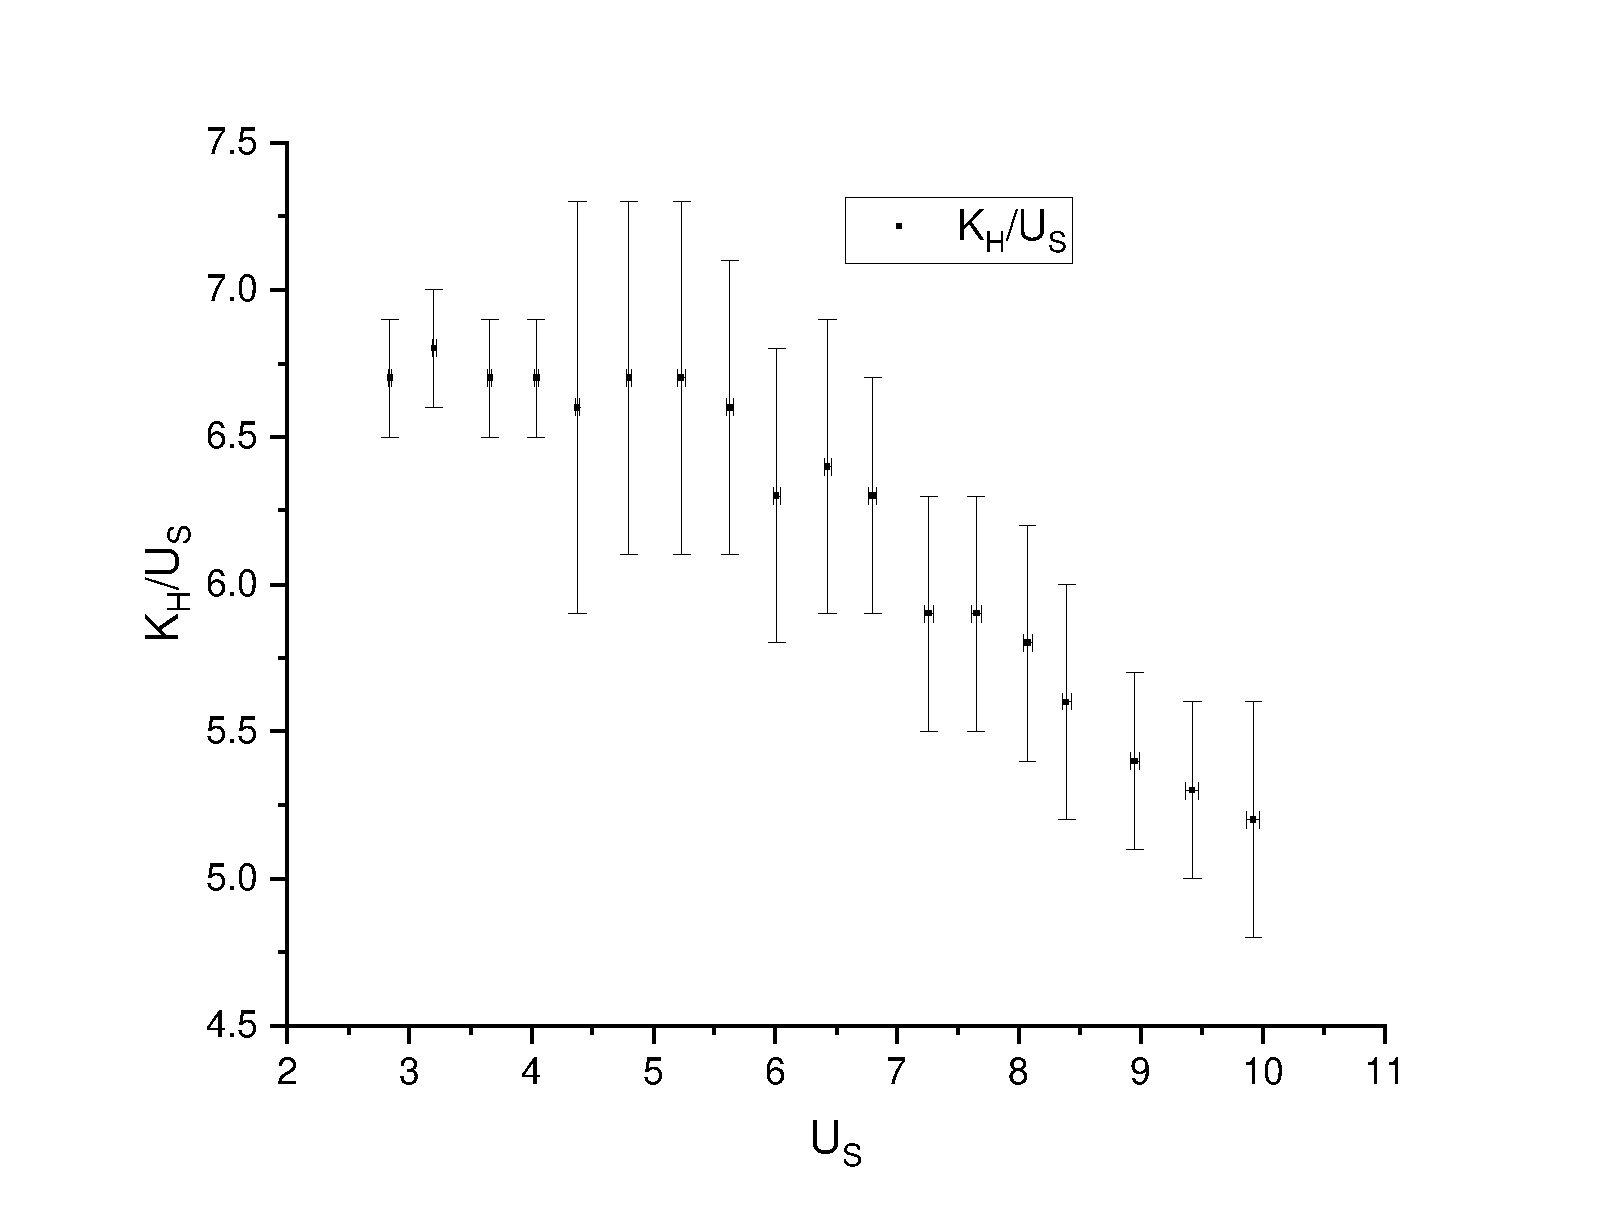
\includegraphics[width=\textwidth]{fig/KHvsUS.pdf}
        \caption{The Relation of $K_H/U_S$ vs. $U_S$}
        \label{fig:KHvsUS}
    \end{figure}
    \subsection{Relation Between Output Voltage $U$ and Magnetic Field $B$}\label{sec:2}
    \paragraph{} Table \ref{tab:origin2} is the original data of the output voltage under different input current. Use the relation $$B=B'I_M/I_0,$$ we can calculate the magnitude of the magnetic field. For example, when $I_M=0.200$[A], $$B=1.4366\times 10^{-3} \times 0.200/0.1=0.00287[\rm T]\pm 0.00006[T].$$
    \begin{table}[H]
        \centering
        \begin{tabular}{|c|c|c|c|}
            \hline
            $I_M$[A]&Uncertainty[A]&$U$[V]&Uncertainty[V]\\\hline
            0&0&0.0000&0.0006\\\hline
            0.0500&0.0010&0.0263&0.0006\\\hline
            0.100&0.002&0.0530&0.0006\\\hline
            0.150&0.003&0.0720&0.0006\\\hline
            0.200&0.004&0.0996&0.0006\\\hline
            0.250&0.005&0.1222&0.0007\\\hline
            0.300&0.006&0.1413&0.0007\\\hline
            0.350&0.007&0.1679&0.0007\\\hline
            0.400&0.008&0.1901&0.0007\\\hline
            0.450&0.009&0.2116&0.0007\\\hline
            0.500&0.010&0.2373&0.0007\\\hline
        \end{tabular}
        \caption{The Original Data}
        \label{tab:origin2}
    \end{table}
    Then I used the data in Table \ref{tab:UvsB} to apply linear fit and got Figure \ref{fig:UvsB}. From it, we can read the slope, whose physical meaning is $K_H$, as $$K_H=32.6[\rm V/T]\pm 0.7[V/T].$$
    \begin{table}[H]
        \centering
        \begin{tabular}{|c|c|c|c|}
            \hline
            $B$[T]&Uncertainty[T]&$U$[V]&Uncertainty[V]\\\hline
            0&0&0.0000&0.0006\\\hline
            0.000718&0.000014&0.0263&0.0006\\\hline
            0.00144&0.00003&0.0530&0.0006\\\hline
            0.00215&0.00004&0.0720&0.0006\\\hline
            0.00287&0.00006&0.0996&0.0006\\\hline
            0.00359&0.00007&0.1222&0.0007\\\hline
            0.00431&0.00009&0.1413&0.0007\\\hline
            0.00503&0.00010&0.1679&0.0007\\\hline
            0.00575&0.00011&0.1901&0.0007\\\hline
            0.00646&0.00013&0.2116&0.0007\\\hline
            0.00718&0.00014&0.2373&0.0007\\\hline
        \end{tabular}
        \caption{The Data for the Linear Fit}
        \label{tab:UvsB}
    \end{table}
    \begin{figure}[H]
        \centering
        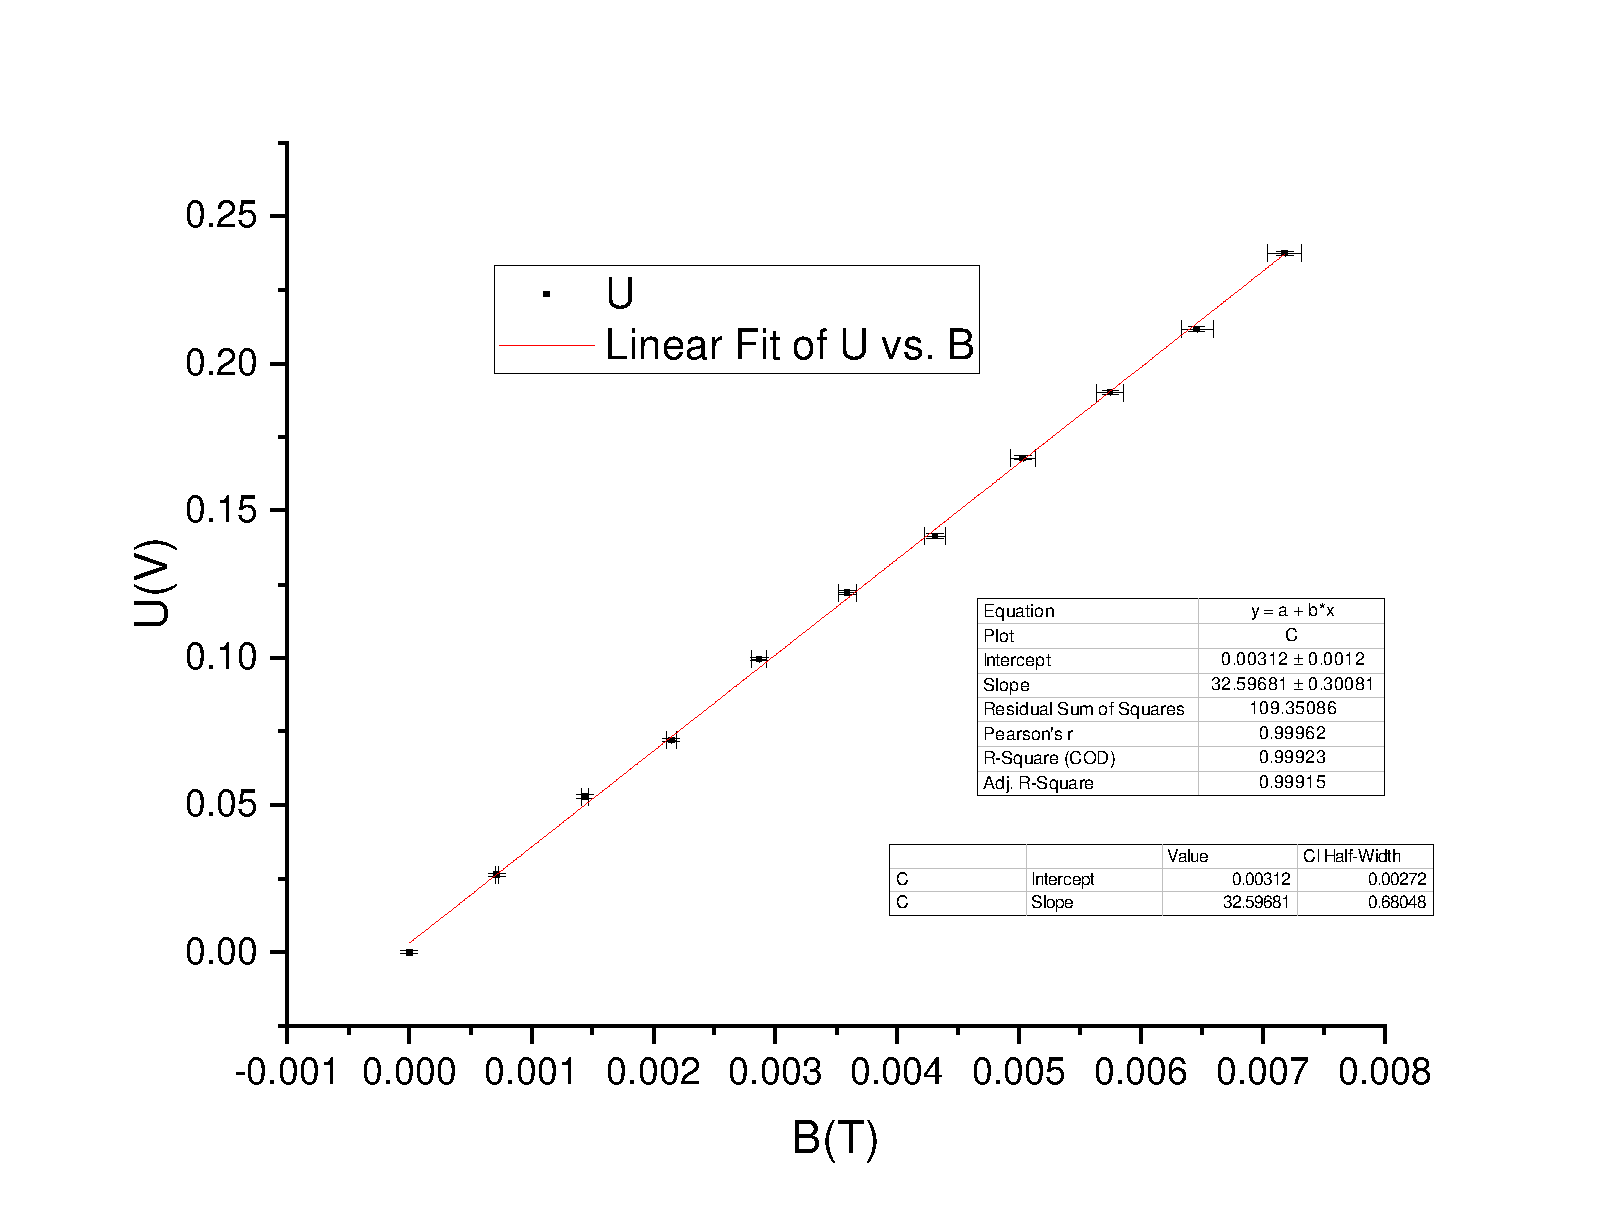
\includegraphics[width=\textwidth]{fig/UvsB.pdf}
        \caption{The Linear Fit of $U$ vs. $B$}
        \label{fig:UvsB}
    \end{figure}
    \subsection{Magnetic Field Distribution Inside the Solenoid}\label{sec:3}
    \begin{table}[H]
        \centering
        \begin{tabular}{|c|c|c|c||c|c|c|c|}
            \hline
            $x$[cm]&Uncertainty[cm]&$U$[V]&Uncertainty[V]&$x$[cm]&Uncertainty[cm]&$U$[V]&Uncertainty[V]\\\hline
            0.00&0.05&0.0097&0.0006&16.00&0.05&0.1219&0.0007\\\hline
            0.50&0.05&0.0131&0.0006&17.00&0.05&0.1222&0.0007\\\hline
            1.00&0.05&0.0178&0.0006&18.00&0.05&0.1223&0.0007\\\hline
            1.50&0.05&0.0253&0.0006&19.00&0.05&0.1223&0.0007\\\hline
            2.00&0.05&0.0367&0.0006&19.50&0.05&0.1220&0.0007\\\hline
            2.50&0.05&0.0510&0.0006&20.00&0.05&0.1219&0.0007\\\hline
            3.00&0.05&0.0689&0.0006&20.50&0.05&0.1218&0.0007\\\hline
            3.50&0.05&0.0852&0.0006&21.00&0.05&0.1216&0.0007\\\hline
            4.00&0.05&0.0969&0.0006&21.50&0.05&0.1214&0.0007\\\hline
            4.50&0.05&0.1043&0.0007&22.00&0.05&0.1210&0.0007\\\hline
            5.00&0.05&0.1093&0.0007&22.50&0.05&0.1207&0.0007\\\hline
            5.50&0.05&0.1129&0.0007&23.00&0.05&0.1204&0.0007\\\hline
            6.00&0.05&0.1152&0.0007&23.50&0.05&0.1198&0.0007\\\hline
            6.50&0.05&0.1170&0.0007&24.00&0.05&0.1190&0.0007\\\hline
            7.00&0.05&0.1183&0.0007&24.50&0.05&0.1180&0.0007\\\hline
            7.50&0.05&0.1191&0.0007&25.00&0.05&0.1168&0.0007\\\hline
            8.00&0.05&0.1198&0.0007&25.50&0.05&0.1151&0.0007\\\hline
            8.50&0.05&0.1202&0.0007&26.00&0.05&0.1130&0.0007\\\hline
            9.00&0.05&0.1208&0.0007&26.50&0.05&0.1096&0.0007\\\hline
            9.50&0.05&0.1211&0.0007&27.00&0.05&0.1047&0.0007\\\hline
            10.00&0.05&0.1214&0.0007&27.50&0.05&0.0975&0.0006\\\hline
            11.00&0.05&0.1218&0.0007&28.00&0.05&0.0866&0.0006\\\hline
            12.00&0.05&0.1219&0.0007&28.50&0.05&0.0704&0.0006\\\hline
            13.00&0.05&0.1220&0.0007&29.00&0.05&0.0524&0.0006\\\hline
            14.00&0.05&0.1218&0.0007&29.50&0.05&0.0354&0.0006\\\hline
            15.00&0.05&0.1216&0.0007&30.00&0.05&0.0258&0.0006\\\hline
        \end{tabular}
        \caption{The Original Data for Section \ref{sec:3}}
        \label{tab:origin3}
    \end{table}
    \paragraph{} Table \ref{tab:origin3} shows the original data of the output voltage for different places inside a solenoid. Since I need to plot a graph with the origin representing the center of the solenoid, and I consider $x=13$[cm] as the center of the solenoid, in Table \ref{tab:exp}, all the value of $x$ are subtracted by 13. For example, if $x=1.00$[cm] in Table \ref{tab:origin3}, $x=1-13=-12.00$[cm] in Table \ref{tab:theoretical}. As for the calculation of the experimental value of $B$, $$B=\frac{U}{K_H},$$ where $K_H=32.6[\rm V/T]\pm 0.7[V/T]$ known from Section \ref{sec:2}. So, for example, when $U=0.0131$[V], $$B=\frac{0.0131}{32.6}=0.40[\rm mT]\pm 0.02[mT].$$
    \begin{table}[H]
        \centering
        \begin{tabular}{|c|c|c|c||c|c|c|c|}
            \hline
            $x$[cm]&$u_x$[cm]&$B$[mT]&$u_B$[mT]&$x$[cm]&$u_x$[cm]&$B$[mT]&$u_B$[mT]\\\hline
            -13.00&0.05&0.298&0.019&3.00&0.05&3.74&0.08\\\hline
            -12.50&0.05&0.40&0.02&4.00&0.05&3.75&0.08\\\hline
            -12.00&0.05&0.55&0.02&5.00&0.05&3.75&0.08\\\hline
            -11.50&0.05&0.78&0.02&6.00&0.05&3.75&0.08\\\hline
            -11.00&0.05&1.13&0.03&6.50&0.05&3.74&0.08\\\hline
            -10.50&0.05&1.56&0.04&7.00&0.05&3.74&0.08\\\hline
            -10.00&0.05&2.11&0.05&7.50&0.05&3.74&0.08\\\hline
            -9.50&0.05&2.61&0.06&8.00&0.05&3.73&0.08\\\hline
            -9.00&0.05&2.97&0.07&8.50&0.05&3.72&0.08\\\hline
            -8.50&0.05&3.20&0.07&9.00&0.05&3.71&0.08\\\hline
            -8.00&0.05&3.35&0.08&9.50&0.05&3.70&0.08\\\hline
            -7.50&0.05&3.46&0.08&10.00&0.05&3.69&0.08\\\hline
            -7.00&0.05&3.53&0.08&10.50&0.05&3.67&0.08\\\hline
            -6.50&0.05&3.59&0.08&11.00&0.05&3.65&0.08\\\hline
            -6.00&0.05&3.63&0.08&11.50&0.05&3.62&0.08\\\hline
            -5.50&0.05&3.65&0.08&12.00&0.05&3.58&0.08\\\hline
            -5.00&0.05&3.67&0.08&12.50&0.05&3.53&0.08\\\hline
            -4.50&0.05&3.69&0.08&13.00&0.05&3.47&0.08\\\hline
            -4.00&0.05&3.71&0.08&13.50&0.05&3.36&0.08\\\hline
            -3.50&0.05&3.71&0.08&14.00&0.05&3.21&0.07\\\hline
            -3.00&0.05&3.72&0.08&14.50&0.05&2.99&0.07\\\hline
            -2.00&0.05&3.74&0.08&15.00&0.05&2.66&0.06\\\hline
            -1.00&0.05&3.74&0.08&15.50&0.05&2.16&0.05\\\hline
            0.00&0.05&3.74&0.08&16.00&0.05&1.61&0.04\\\hline
            1.00&0.05&3.74&0.08&16.50&0.05&1.09&0.03\\\hline
            2.00&0.05&3.73&0.08&17.00&0.05&0.79&0.03\\\hline
        \end{tabular}
        \caption{The Experimental Result of $B$ vs. $x$}
        \label{tab:exp}
    \end{table}
    \paragraph{}Also, we need to calculate the theoretical value of $B$ when $I_M=0.25$[A]. $B=B'I_M/I_0$, where $B'$ is the value in Table \ref{tab:theoretical} and $I_0=0.1$[A]. For example, when $B'=1.4366$[mT], $$B=\frac{1.4366\times 0.25}{0.1}=3.59[\rm mT]\pm 0.07[mT].$$ Table \ref{tab:theory} shows the theoretical value of $B$ vs. $x$ when $I_M=250$[mA] using data in Table \ref{tab:theoretical}. Then I used the data in Table \ref{tab:exp} and \ref{tab:theory} to plot Figure \ref{fig:Bvsx}, which is the magnetic field inside a solenoid.
    \begin{table}[H]
        \centering
        \begin{tabular}{|c|c|c|}
            \hline
            $x$[cm]&$B$[mT]&Uncertainty[mT]\\\hline
            $\pm 0.0$&3.59&0.07\\\hline
            $\pm 1.0$&3.59&0.07\\\hline
            $\pm 2.0$&3.59&0.07\\\hline
            $\pm 3.0$&3.59&0.07\\\hline
            $\pm 4.0$&3.58&0.07\\\hline
            $\pm 5.0$&3.57&0.07\\\hline
            $\pm 6.0$&3.56&0.07\\\hline
            $\pm 7.0$&3.54&0.07\\\hline
            $\pm 8.0$&3.51&0.07\\\hline
            $\pm 9.0$&3.46&0.07\\\hline
            $\pm 10.0$&3.37&0.07\\\hline
            $\pm 11.0$&3.17&0.06\\\hline
            $\pm 11.5$&2.99&0.06\\\hline
            $\pm 12.0$&2.72&0.05\\\hline
            $\pm 12.5$&2.32&0.05\\\hline
            $\pm 13.0$&1.81&0.04\\\hline
        \end{tabular}
        \caption{The Theoretical Result of $B$ vs. $x$}
        \label{tab:theory}
    \end{table}
    \begin{figure}[H]
        \centering
        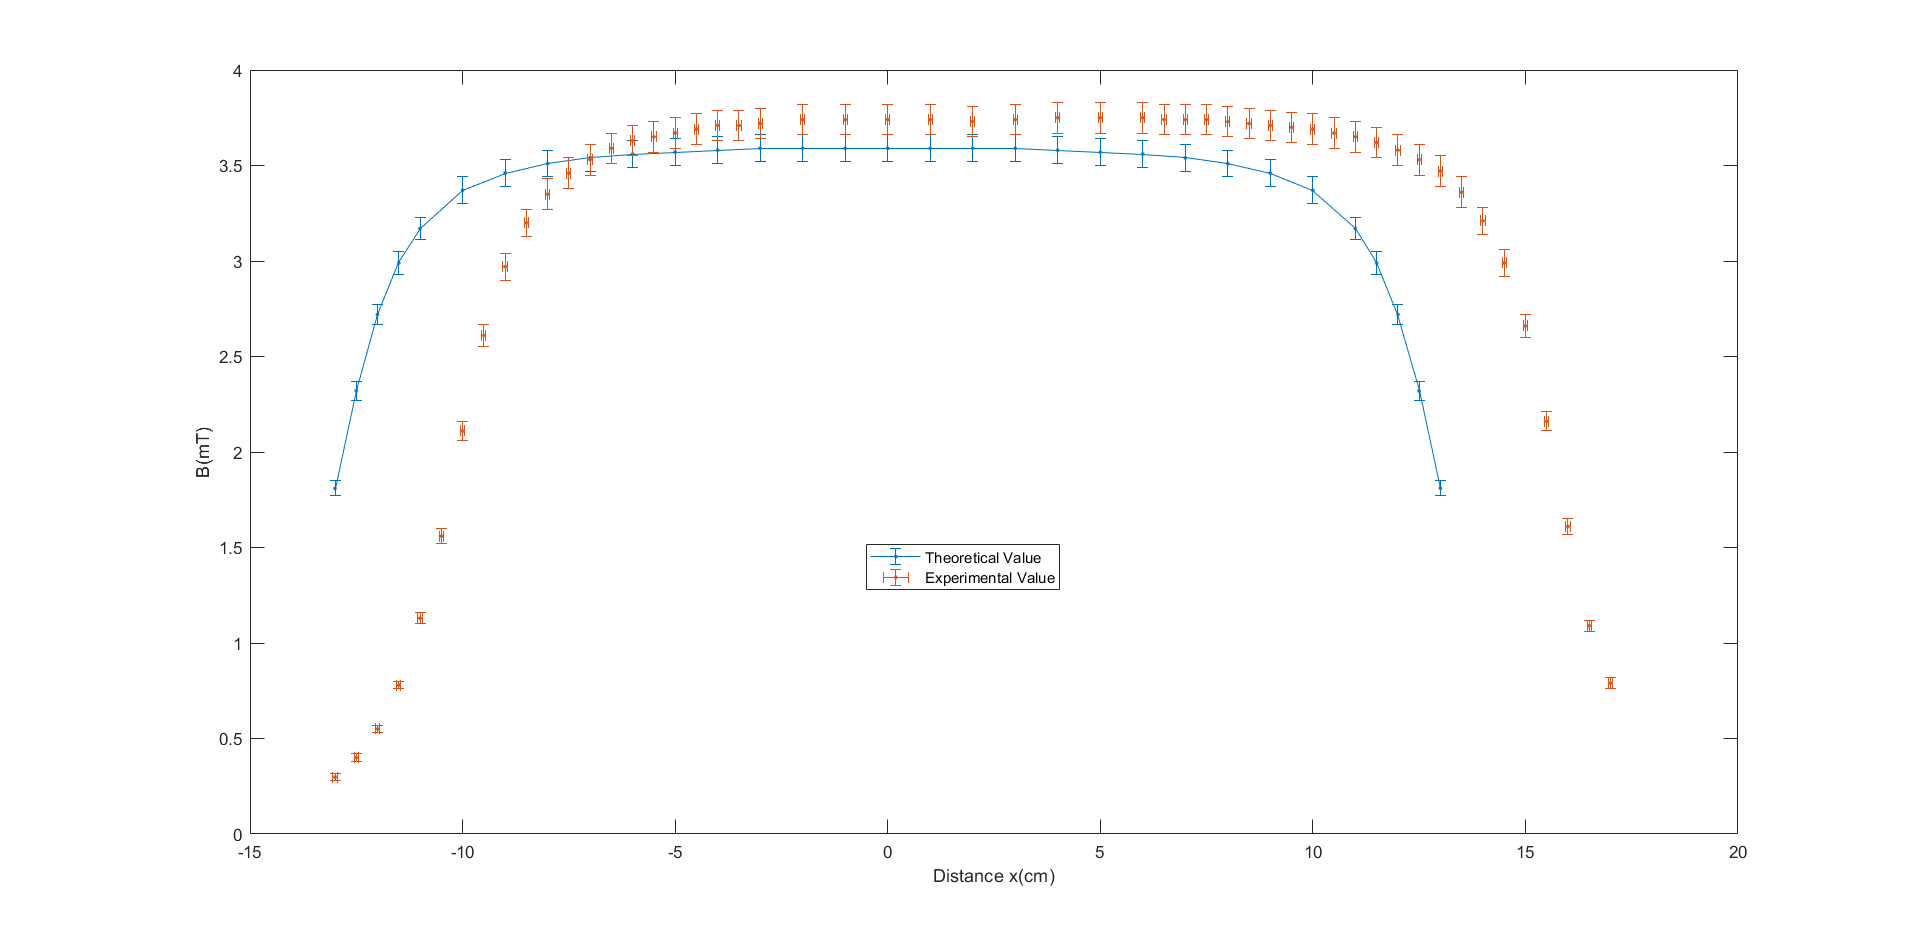
\includegraphics[width=\textwidth]{fig/Bvsx.png}
        \caption{The Theoretical and Experimental Magnetic Field inside a Solenoid}
        \label{fig:Bvsx}
    \end{figure}
    \section{Discussion}
    \paragraph{} In the first part of this lab, we measure the Hall sensitivity $K_H$ under working voltage $U_S=5$[V]. We get \begin{equation*}
        \begin{split}
            K_H^*=35[{\rm V/T}]\pm 3[{\rm V/T}]\\
            K_{H,t}=31.25[\rm V/T]\pm 1.25[V/T]
        \end{split}
    \end{equation*}
    We can see that although the value of $K_H^*$ and $K_H$(theoretical) is within the uncertainty of each other, the uncertainty of $K_H^*$ is rather huge. Also, we have obtained $$K_H=32.6[\rm V/T]\pm 0.7[V/T]$$ from the second part of this lab through linear fit. All of these three values lie in the range of one another's uncertainty, but $K_H$ clearly has a smaller uncertainty than $K_H^*$. And that is why I used $K_H$ instead of $K_H^*$ in the third part to calculate the experimental value of $B$.
    \vspace{-5mm}
    \paragraph{} In the first part, we have measured $K_H$ under different working voltage $U_S$ and obtained Figure \ref{fig:KHvsUS}. From this figure, we can not see any pattern between $K_H$ and $U_S$. But I can conclude that under different working voltage, $K_H$ tends to be different. Also, from Table \ref{tab:KHvsUS}, the trend is that the higher the working voltage, the large the $K_H$.
    \vspace{-5mm}
    \paragraph{} In the third part of the experiment, I obtained both theoretical and experimental values of $B$ in different positions inside a solenoid and plotted Figure \ref{fig:Bvsx}. If we view the two sets of data separately (either experimental or theoretical), we can conclude that there is a range near the center of the solenoid where the magnetic field is uniform, while it decreases as we approach either end of the solenoid. However, the starting and ending point of the uniform magnetic field is different for the theoretical and experimental value. The reason might be that the center of the solenoid should be $15$[cm] instead of 13[cm]. Also, the magnitude of the uniform magnetic field is different. The reason is probably that the $K_H$ I used to calculate the experimental values is larger than the actual $K_H$.
    \section{Conclusion}
    \paragraph{} In this lab, we have measured the Hall sensitivity of the Hall probe under different working voltages. Also, we have obtained two experimental value of $K_H$ using two methods. One is direct measurement and the other is linear fit. In addition, we have measured the magnetic field inside a solenoid. All these three experiments are very successful as no results deviates from the theoretical values too much. However, it is unsatisfactory that some of the values (such as $K_H^*$) have very large uncertainty. In order to optimize the result and have more accurate data, here are some suggestions: 
    \begin{enumerate}
        \item Change for better equipment, especially the voltage source. During the experiment, the output voltage kept increasing bit by bit after I stopped touch the knob, which made the reading on the multimeter keep changing, which causes much trouble for reading.
        \item We can measure the output voltage several time when measuring $K_H^*$, which can minimize the effect of Type-A uncertainty.
    \end{enumerate}
    \section{Reference}
    \begin{enumerate}
        \item Qin Tian, Wang Zhiyu, Lin Yiqiao, Mateusz Krzyzosiak, ``Exercise 2- lab manual [rev. 3.8]''.
    \end{enumerate}
    \renewcommand\thesection{\Alph{section}} 
    \setcounter{section}{0}
    \newpage
    \section{Uncertainty Analysis}
    \subsection{The Uncertainty of the Voltages in Section \ref{sec:1}}
    \paragraph{} We first calculate the uncertainty in table \ref{tab:origin1}. For the uncertainty of $U_S$, $u=U_S\times 0.5\%$. For example, when $U_S=2.84$[V], $$u=U_S\times 0.5\%=2.84 \times 0.5\%=0.014[\rm V].$$
    \paragraph{} Then the uncertainty of $U_0$ and $U$. $u=U\times 0.05\%+6\times 10^{-3} \text{ or }6\times 10^{-4}$. For instance, when $U_0=1.4004$[V], $$u=1.4004\times 0.05\%+0.0006=0.0013[\rm V].$$ When $U=2.266$[V], $$u=2.266\times 0.05\%+0.006=0.007[\rm V].$$
    \subsection{The Uncertainty of the Magnetic Field in Section \ref{sec:1}}
    \paragraph{} As we know, $$B=B'\frac{I}{I_0}.$$ where $B'=1.4366$[mT], $I_0=0.1$[A], $I=0.25$[A], $u_I=I\times 2\%=0.005$[A], and the uncertainty of both $B'$ and $I_0$ is zero because these data are theoretical values. Then the uncertainty of the calculated magnetic field is $$u_B=\left|\frac{\partial B}{\partial I}u_I\right|=\frac{B'}{I_0}u_I=\frac{1.4366\times 10^{-3}}{0.1}\times 0.005=0.00007[\rm T].$$
    \subsection{The Uncertainty of $K_H$ and $K_H/U_S$ in Section \ref{sec:1}}
    \paragraph{} Since $K_H=\frac{U-U_0}{B}$, the uncertainty can be calculated as \begin{equation*}
        \begin{split}
            u&=\sqrt{\left(\frac{\partial K_H}{\partial U}u_U\right)^2+\left(\frac{\partial K_H}{\partial B}u_B\right)^2+\left(\frac{\partial K_H}{\partial U_0}u_{U_0}\right)^2}\\
            &=\sqrt{\frac{u_U^2}{B^2}+\frac{u_{U_0}^2}{B^2}+\frac{(U-U_0)^2u_B^2}{B^4}}\\
            &=\frac{1}{B^2}\sqrt{(u_U^2+u_{U_0}^2)B^2+(U-U_0)^2u_B^2}.
        \end{split}
    \end{equation*}
    For example, when $B=0.00359$[T], $U=1.4689$[V], $U_0=1.4004$[V], $u_B=0.00007$[T], $u_U=0.0013$[V], $u_{U_0}=0.0013$[V], then the uncertainty of $K_H$ is $$u=\frac{1}{0.00359^2}\sqrt{(2\times 0.0013^2)\times 0.00359^2+(1.4689-1.4004)^2\times 0.00007^2}=0.6[\rm V/T].$$
    The same calculation can be applied to the uncertainty of $K_H^*$.
    \vspace{-5mm}
    \paragraph{} As for the uncertainty of $K_H/U_S$, \begin{equation*}
        \begin{split}
            u&=\sqrt{\left(\frac{\partial}{\partial K_H}\left(\frac{K_H}{U_S}\right)u_{K_H}\right)^2+\left(\frac{\partial}{\partial U_S}\left(\frac{K_H}{U_S}\right)u_{U_S}\right)^2}\\
            &=\sqrt{\frac{u_{K_H}^2}{U_S^2}+\frac{K_H^2u_{U_S}^2}{U_S^4}}\\
            &=\frac{1}{U_S^2}\sqrt{u_{K_H}^2U_S^2+K_H^2u_{U_S}^2}.
        \end{split}
    \end{equation*} 
    So, when $K_H=19.1$[V/T], $U_S=2.84$[V], $u_{K_H}=0.6$[V/T], $u_{U_S}=0.014$[V], we have $$u=\frac{1}{2.84^2}\times\sqrt{0.6^2\times 2.84^2+19.1^2\times 0.014^2}=0.2[{\rm T}^{-1}].$$
    \subsection{The Uncertainty of $I_M$, $U$ and $B$ in Section \ref{sec:2}}
    \paragraph{} The uncertainty for $I_M$ is $u=I_M\times 2\%$[A]. So, for example, when $I_M=0.1$[A], $$u=0.1\times 2\%=0.002[\rm A].$$ 
    \paragraph{} The uncertainty for $U$ is $u=U\times 0.05\%+0.0006$[V]. So, when $U=52.97$[mV], $$u=52.97/1000\times 0.05\%+0.0006=0.0006[\rm V].$$
    \paragraph{} Since $B=B'I_M/I_0$, where $I_0=0.1$A and $B'=1.4366\times 10^{-3}$T, the uncertainty of the magnetic field is $$u=\left|\frac{\partial B}{\partial I_M}u_{I_M}\right|=\frac{B'u_{I_M}}{I_0}.$$ For example, when $I_M=0.1$[A], $u_{I_M}=0.002$[A], $$u=\frac{1.4366\times 10^{-3}\times 0.002}{0.1}=0.00003[\rm T].$$
    \subsection{The Uncertainty of the experimental and theoretical magnetic field $B$ in Section \ref{sec:3}}
    \paragraph{} The uncertainty of the voltages is $u=U\times 0.05\% +0.0006$[V]. For example, when $U=0.0131$[V], $$u=0.0131\times 0.05\%+0.0006=0.0006[\rm V]$$  
    \paragraph{} We then calculate the uncertainty of the experimental value of $B$. Since here $B=U/K_H$, we have \begin{equation*}
        \begin{split}
            u&=\sqrt{\left(\frac{\partial B}{\partial U}u_U\right)^2+\left(\frac{\partial B}{\partial K_H}u_{K_H}\right)^2}\\
            &=\sqrt{\frac{u_U^2}{K_H^2}+\frac{U^2u_{K_H}^2}{K_H^4}}\\
            &=\frac{1}{K_H^2}\sqrt{u_U^2K_H^2+U^2u_{K_H}^2}.
        \end{split}
    \end{equation*}
    Here we use the experimental value of $K_H$, which was obtained in Section \ref{sec:2}: $K_H=32.6$[V/T], $u_{K_H}=0.7$[V/T]. For example, when $U=0.0131$[V], $u_U=0.0006$[V],$$u=\frac{1}{32.6^2}\times \sqrt{0.0006^2\times 32.6^2+0.0131^2\times 0.7^2}=0.00002[\rm T]=0.02[mT].$$
    \paragraph{} As for the theoretical value of the magnetic field, $B_t=B'I_M/I_0$, where $I_0=0.1$A, and $B'$ is the value listed in Table \ref{tab:theoretical}, so the uncertainty is $$u=\left|\frac{\partial B_t}{\partial I_M}u_{I_M}\right|=\frac{B'u_{I_M}}{I_0}.$$ Here, $u_{I_M}=0.25\times 2\%=0.005$[A]. For example, when $B'=1.4366[mT]$, $$u=\frac{1.4366\times 0.005}{0.1}=0.07[\rm mT].$$
    \section{Data Sheet}
    \paragraph{} The data sheets are attached to this report.
\end{document}